\begin{figure}[H]
\centering
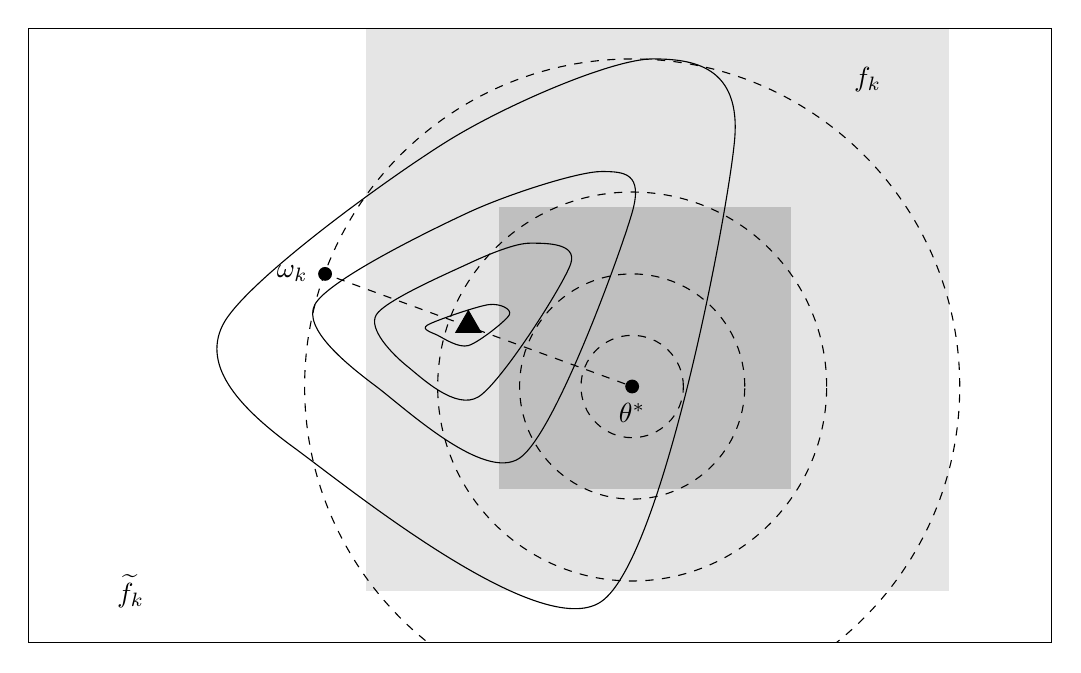
\begin{tikzpicture}[scale=1.3]
% \coordinate (origin) at (0, 0);
\fill [gray!20] (-1.7, -2.5) rectangle (4, 3);
\fill [gray!50] (-0.4, -1.5) rectangle (2.45, 1.25);
\draw (-5, -3) rectangle (5, 3);
\node at (3.2,2.5) {$\dom f_k$};
\node at (-4,-2.5) {$\widetilde{\dom f_k}$};
\draw[] plot [smooth cycle] coordinates {(-1, 0) (-0.7, -0.1) (-0.3, 0.2) (-0.5, 0.3) (-1.1, 0.1)};
\draw[] plot [smooth cycle] coordinates {(-1.3, -0.3) (-0.6, -0.6) (0.3, 0.7) (-0.1, 0.9) (-0.7, 0.7) (-1.6, 0.2)};
\draw[] plot [smooth cycle] coordinates {(-1.6, -0.5) (-0.2, -1.2) (0.9, 1.2) (0.6, 1.6) (-0.7, 1.2) (-2.2, 0.3)};
\draw[] plot [smooth cycle] coordinates {(-2.4, -1.1) (0.6, -2.6) (1.9, 1.9) (1.1, 2.7) (-0.9, 1.9) (-3.1, 0.1)};
\node at (0.9, -0.5) (theta) [circle,fill=black,inner sep=0pt,minimum size=5pt,label=below:{$\theta^*$}] {};
\node at (-2.1, 0.6) (omega1) [circle,fill=black,inner sep=0pt,minimum size=5pt,label=left:{$\omega_k$}] {};
\draw[dashed, thin] (theta) -- (omega1);
\draw plot[only marks, mark=triangle*, mark size=4pt, thick] coordinates {(-0.7, 0.1)};
\begin{scope}
\clip (-5, -3) rectangle (5, 3);
\draw[dashed, thin] (theta) circle (0.5);
\draw[dashed, thin] (theta) circle (1.1);
\draw[dashed, thin] (theta) circle (1.9);
\draw[dashed, thin] (theta) circle (3.2);
\end{scope}
\end{tikzpicture}
\caption{$f_k(\alpha_k \omega_k + (1 - \alpha_k) \theta^*)$的示意图}
\label{fig:apfl}
\end{figure}
